\documentclass{article}
\usepackage{tikz}
\usetikzlibrary{positioning}

\begin{document}

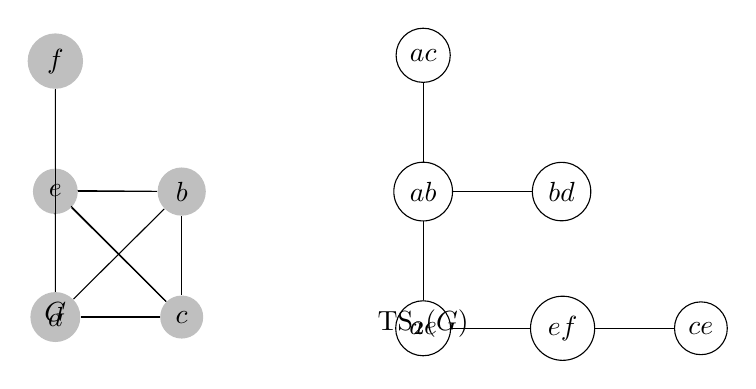
\begin{tikzpicture}[node distance=1cm]
    % Define nodes for graph G
    \node[circle, fill=gray!50] (a) at (0,0) {$a$};
    \node[circle, fill=gray!50, right=of a] (b) {$b$};
    \node[circle, fill=gray!50, below=of b] (c) {$c$};
    \node[circle, fill=gray!50, left=of c] (d) {$d$};
    \node[circle, fill=gray!50, above=of d] (e) {$e$};
    \node[circle, fill=gray!50, above=of e] (f) {$f$};

    % Draw edges for graph G
    \draw (a) -- (b);
    \draw (a) -- (c);
    \draw (a) -- (d);
    \draw (a) -- (e);
    \draw (a) -- (f);
    \draw (b) -- (c);
    \draw (b) -- (d);
    \draw (b) -- (e);
    \draw (c) -- (d);
    \draw (c) -- (e);
    \draw (d) -- (e);
    \draw (d) -- (f);
    \draw (e) -- (f);

    % Label the graph G
    \node[below=1cm of a] {$G$};

    % Define nodes for TS_2(G)
    \node[circle, draw, right=4cm of a] (ab) {$ab$};
    \node[circle, draw, above=1cm of ab] (ac) {$ac$};
    \node[circle, draw, right=1cm of ab] (bd) {$bd$};
    \node[circle, draw, below=1cm of ab] (ae) {$ae$};
    \node[circle, draw, right=1cm of ae] (ef) {$ef$};
    \node[circle, draw, right=1cm of ef] (ce) {$ce$};

    % Draw edges for TS_2(G)
    \draw (ab) -- (ac);
    \draw (ab) -- (bd);
    \draw (ab) -- (ae);
    \draw (ae) -- (ef);
    \draw (ef) -- (ce);

    % Label the TS_2(G)
    \node[below=1cm of ab] {$\mathrm{TS}_2(G)$};
\end{tikzpicture}

\end{document}